\documentclass[11pt]{article}

\usepackage[margin=1in]{geometry}
\usepackage{booktabs}
\usepackage{siunitx}
\usepackage{tikz}
\usepackage{xcolor}

\sisetup{round-mode=places, round-precision=2, group-digits=integer}

\title{Per-stage runtime of the four-index BIE pipeline\\
on the graphene-monolayer system (precompute-once volume field)}
\author{Numerical experiment 6.5 --- exp65\_orbital\_bench}
\date{2026-06-15}

\begin{document}
\maketitle

\section{Setup}

Single right-hand-side solve of the screened-Coulomb four-index integral on
the real graphene monolayer (Wannier $p_z$ orbital, $k_{323201}$), using the
production pipeline with the \texttt{PrecomputedVolumeField} (\texttt{cache\_fft})
volume-field method for the volume-potential stages. All timings are warm
(post-JIT), measured on a single idle node.

\begin{table}[h]
\centering
\begin{tabular}{ll}
\toprule
\multicolumn{2}{l}{\textbf{Hardware / software}}\\
\midrule
CPU            & $2\times$ AMD EPYC 9474F (96 cores), 96 threads\\
Memory         & \SI{1.5}{\tera\byte} (peak RSS \SI{29.4}{\giga\byte})\\
OS / kernel    & Rocky Linux 8.10, kernel 6.6\\
Julia          & 1.12.6\\
Libraries      & FINUFFT.jl 3.5.2, finufft\_jll 2.5.1, FMM3D\\
\midrule
\multicolumn{2}{l}{\textbf{Problem}}\\
\midrule
Geometry       & slab $L\times L\times L_z = 90\times90\times3.35$, $\varepsilon_{\mathrm{in}}=3.5$\\
Source         & squared $p_z$ orbital, \num{355862} grid points\\
Tolerances     & source/RHS $10^{-3}$, LHS/eval $10^{-5}$, GMRES $10^{-5}$\\
Discretization & $n_{\mathrm{quad}}=6$, edge level $4$, edge correction on\\
Interface      & \num{960768} points; GMRES 8 iters, residual \num{7.1e-6}\\
Result         & $u_{\mathrm{onsite}} = \SI{9.88}{\electronvolt}$\\
\bottomrule
\end{tabular}
\end{table}

\section{Per-stage runtime}

\begin{table}[h]
\centering
\begin{tabular}{l l S[table-format=2.2]}
\toprule
\textbf{Phase} & \textbf{Stage} & {\textbf{Time (s)}}\\
\midrule
Load        & XSF read $+$ truncation $+$ screening      & 3.25\\
\addlinespace
Precompute  & Field construction (\texttt{cache\_fft})    & 8.82\\
Precompute  & Interface build (RHS-adaptive)              & 6.76\\
Precompute  & LHS assembly (near corrections)             & 13.56\\
\addlinespace
Solve       & RHS assembly (field)                        & 2.18\\
Solve       & GMRES solve (8 iterations)                  & 22.21\\
\addlinespace
Eval        & Volume potential $u_{\mathrm{int}}$ (field) & 0.12\\
Eval        & Scattered potential (FMM $+$ cubature)      & 5.38\\
\midrule
\textbf{Total} & & 62.28\\
\bottomrule
\end{tabular}
\caption{Wall-clock time per pipeline stage (warm, 96 threads).}
\end{table}

\begin{table}[h]
\centering
\begin{tabular}{l S[table-format=2.2] S[table-format=2.1]}
\toprule
\textbf{Phase} & {\textbf{Time (s)}} & {\textbf{Share (\%)}}\\
\midrule
Load                                & 3.25  & 5.2\\
Precompute (construct $+$ build $+$ LHS) & 29.14 & 46.8\\
Solve (RHS $+$ GMRES)               & 24.39 & 39.2\\
Eval ($u_{\mathrm{int}}$ $+$ scatter) & 5.50  & 8.8\\
\midrule
\textbf{Total}                      & 62.28 & 100.0\\
\bottomrule
\end{tabular}
\caption{Phase totals.}
\end{table}

\begin{figure}[h]
\centering
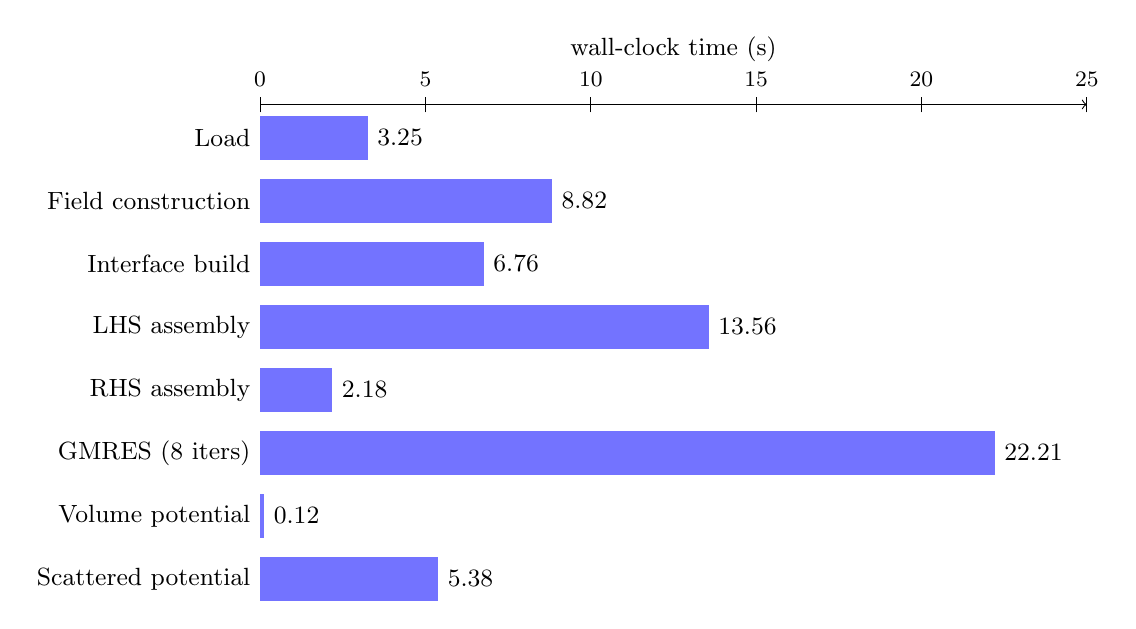
\begin{tikzpicture}[x=0.42cm, y=1cm]
  % horizontal bars: row i at y = -0.8*i, bar from x=0 to x=time (seconds)
  \foreach \time/\lab/\i in {%
      3.25/{Load}/0,
      8.82/{Field construction}/1,
      6.76/{Interface build}/2,
      13.56/{LHS assembly}/3,
      2.18/{RHS assembly}/4,
      22.21/{GMRES (8 iters)}/5,
      0.12/{Volume potential}/6,
      5.38/{Scattered potential}/7}
  {
    \fill[blue!55] (0,{-0.8*\i}) rectangle (\time,{-0.8*\i+0.55});
    \node[left, font=\small] at (0,{-0.8*\i+0.275}) {\lab};
    \node[right, font=\small] at (\time,{-0.8*\i+0.275}) {\time};
  }
  % axis
  \draw[->] (0,0.7) -- (25,0.7);
  \foreach \t in {0,5,10,15,20,25}
    {\draw (\t,0.6) -- (\t,0.8); \node[above, font=\footnotesize] at (\t,0.8) {\t};}
  \node[font=\small] at (12.5,1.4) {wall-clock time (s)};
\end{tikzpicture}
\caption{Per-stage wall-clock time. The pipeline is dominated by GMRES,
LHS assembly, and the one-time field construction; the volume-potential
evaluation ($u_{\mathrm{int}}$) is essentially free.}
\end{figure}

\section{Notes}

\begin{itemize}
\item \textbf{Dominant costs} are GMRES (\SI{22.2}{\second}), LHS assembly
      (\SI{13.6}{\second}), field construction (\SI{8.8}{\second}), and the
      interface build (\SI{6.8}{\second}); the pipeline is solve/assembly-bound.
\item \textbf{Amortization.} The RHS-independent precompute (field
      construction $+$ interface build $+$ LHS assembly $=\SI{29.1}{\second}$)
      is paid once. Each additional right-hand side on the same
      geometry/source family costs RHS $+$ GMRES $+$ eval $\approx
      \SI{30}{\second}$, dominated by GMRES.
\item \textbf{Volume field.} The precomputed spectral field is reused across
      all mesh-refinement depths and the evaluation; with \texttt{cache\_fft}
      the $u_{\mathrm{int}}$ read-out is interpolation-only
      (\SI{0.12}{\second}).
\item \textbf{Memory.} Peak RSS \SI{29.4}{\giga\byte}, set by the
      \texttt{cache\_fft} fine-grid storage; the standard field
      (\texttt{cache\_fft = false}) peaks at $\sim\SI{14}{\giga\byte}$ with
      $u_{\mathrm{int}}\approx\SI{0.4}{\second}$.
\end{itemize}

\end{document}
